\documentclass[../main.tex]{subfiles}
\graphicspath{{\subfix{./figs/}}}
% fix energy of figures

\begin{document}

\section{Generated Distributions}
An example of both a h---h and h---$\Lambda$ correlation, generated from our PYTHIA6 events, are shown in Fig. \ref{fig:hh08} and Fig. \ref{fig:hl08}, respectively. We also include projections of relevant kinematic variables to demonstrate the cuts used to construct an angular correlation. All fits are shown in Appendix \ref{appendix:a}. 

\begin{figure}[h]
    \centering
    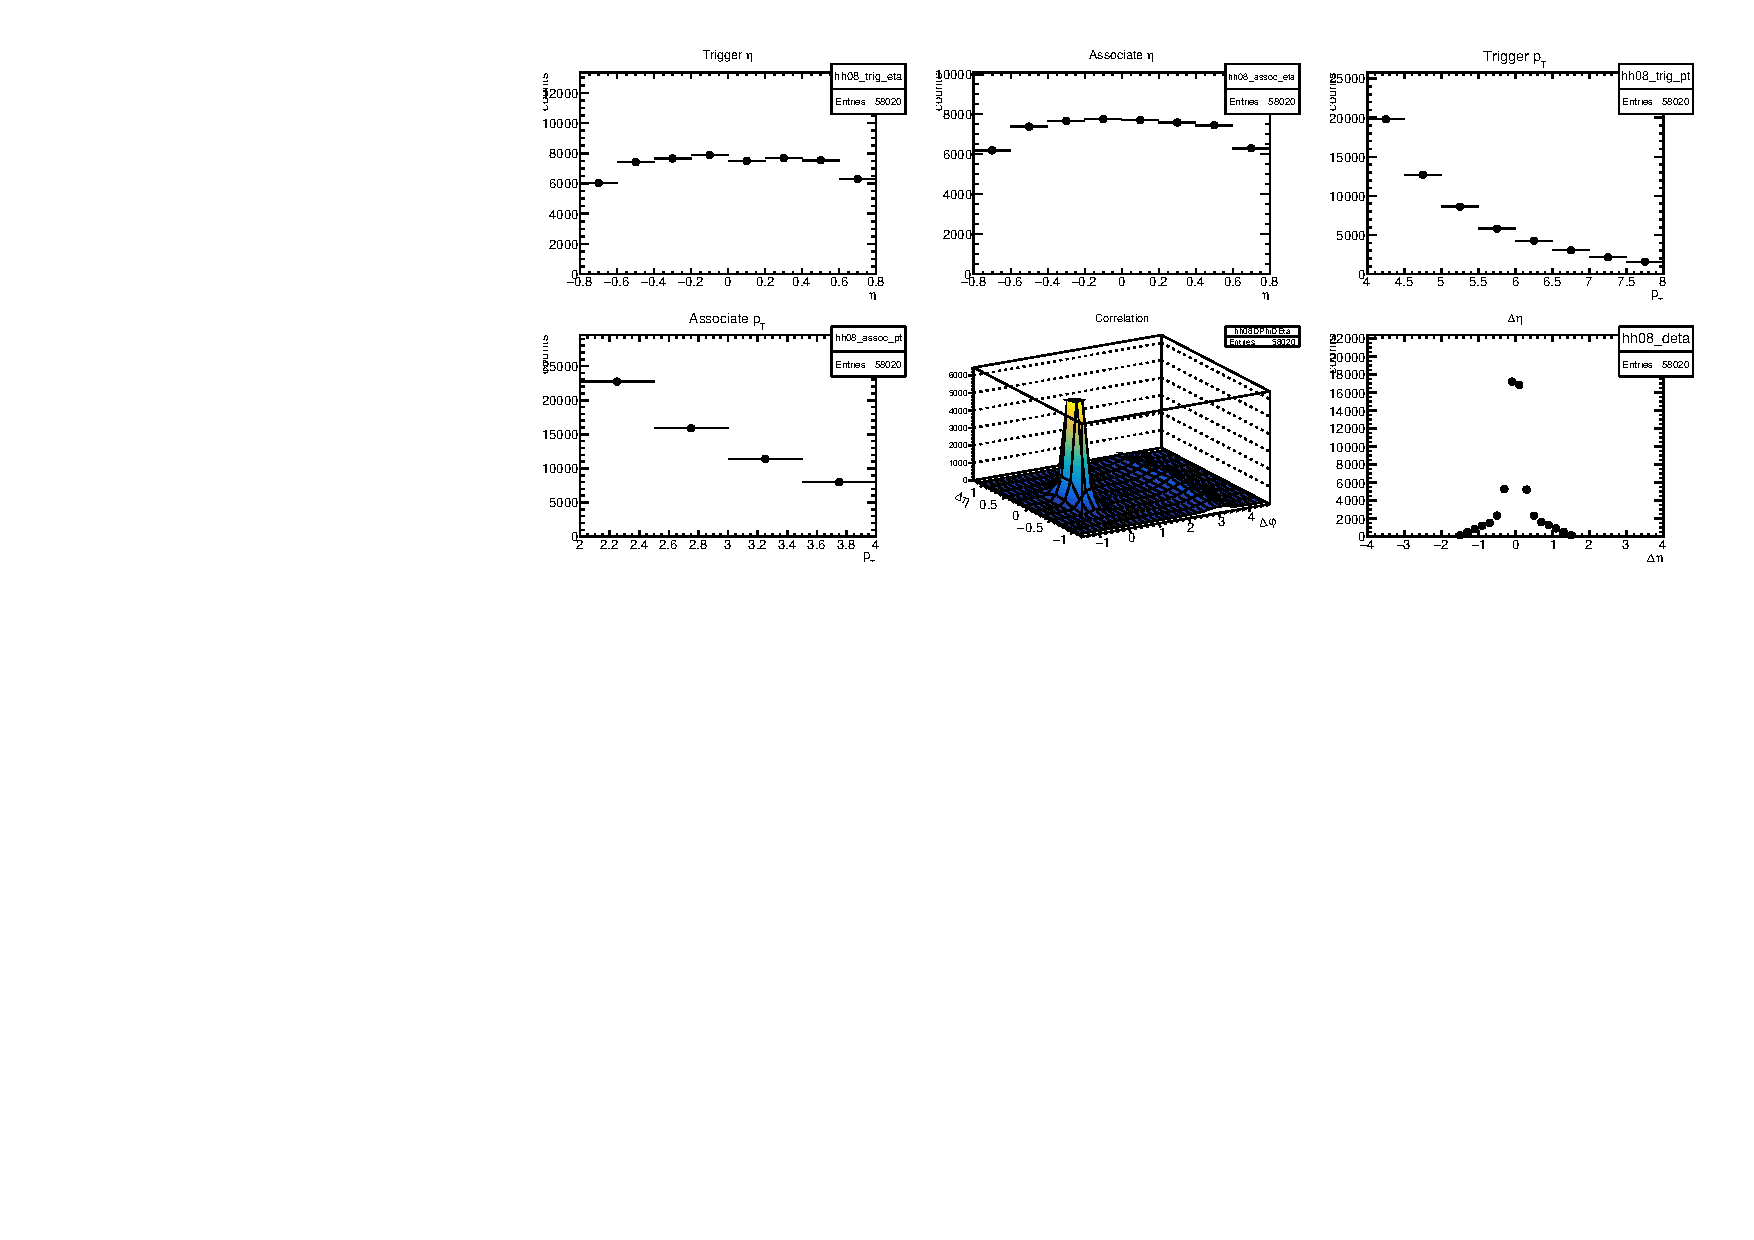
\includegraphics[scale=0.9]{results/figs/hh08_projections.pdf}
    \caption{A h---h correlation for $2 < p_T^{\text{assoc}} < 4$, $4<p_T^{\text{assoc}}<8$, and $|\eta|<0.8$. All single-particle distributions are constructed from particles that are counted in the 2D angular correlation. We see the $\eta$ distributions are abruptly cut off at $\eta = \pm 0.8$, and the $p_T$ distributions also display cuts. The $\Delta \eta$ distribution is a projection of the 2D angular correlation.}
    \label{fig:hh08}
\end{figure}

\begin{figure}
    \centering
    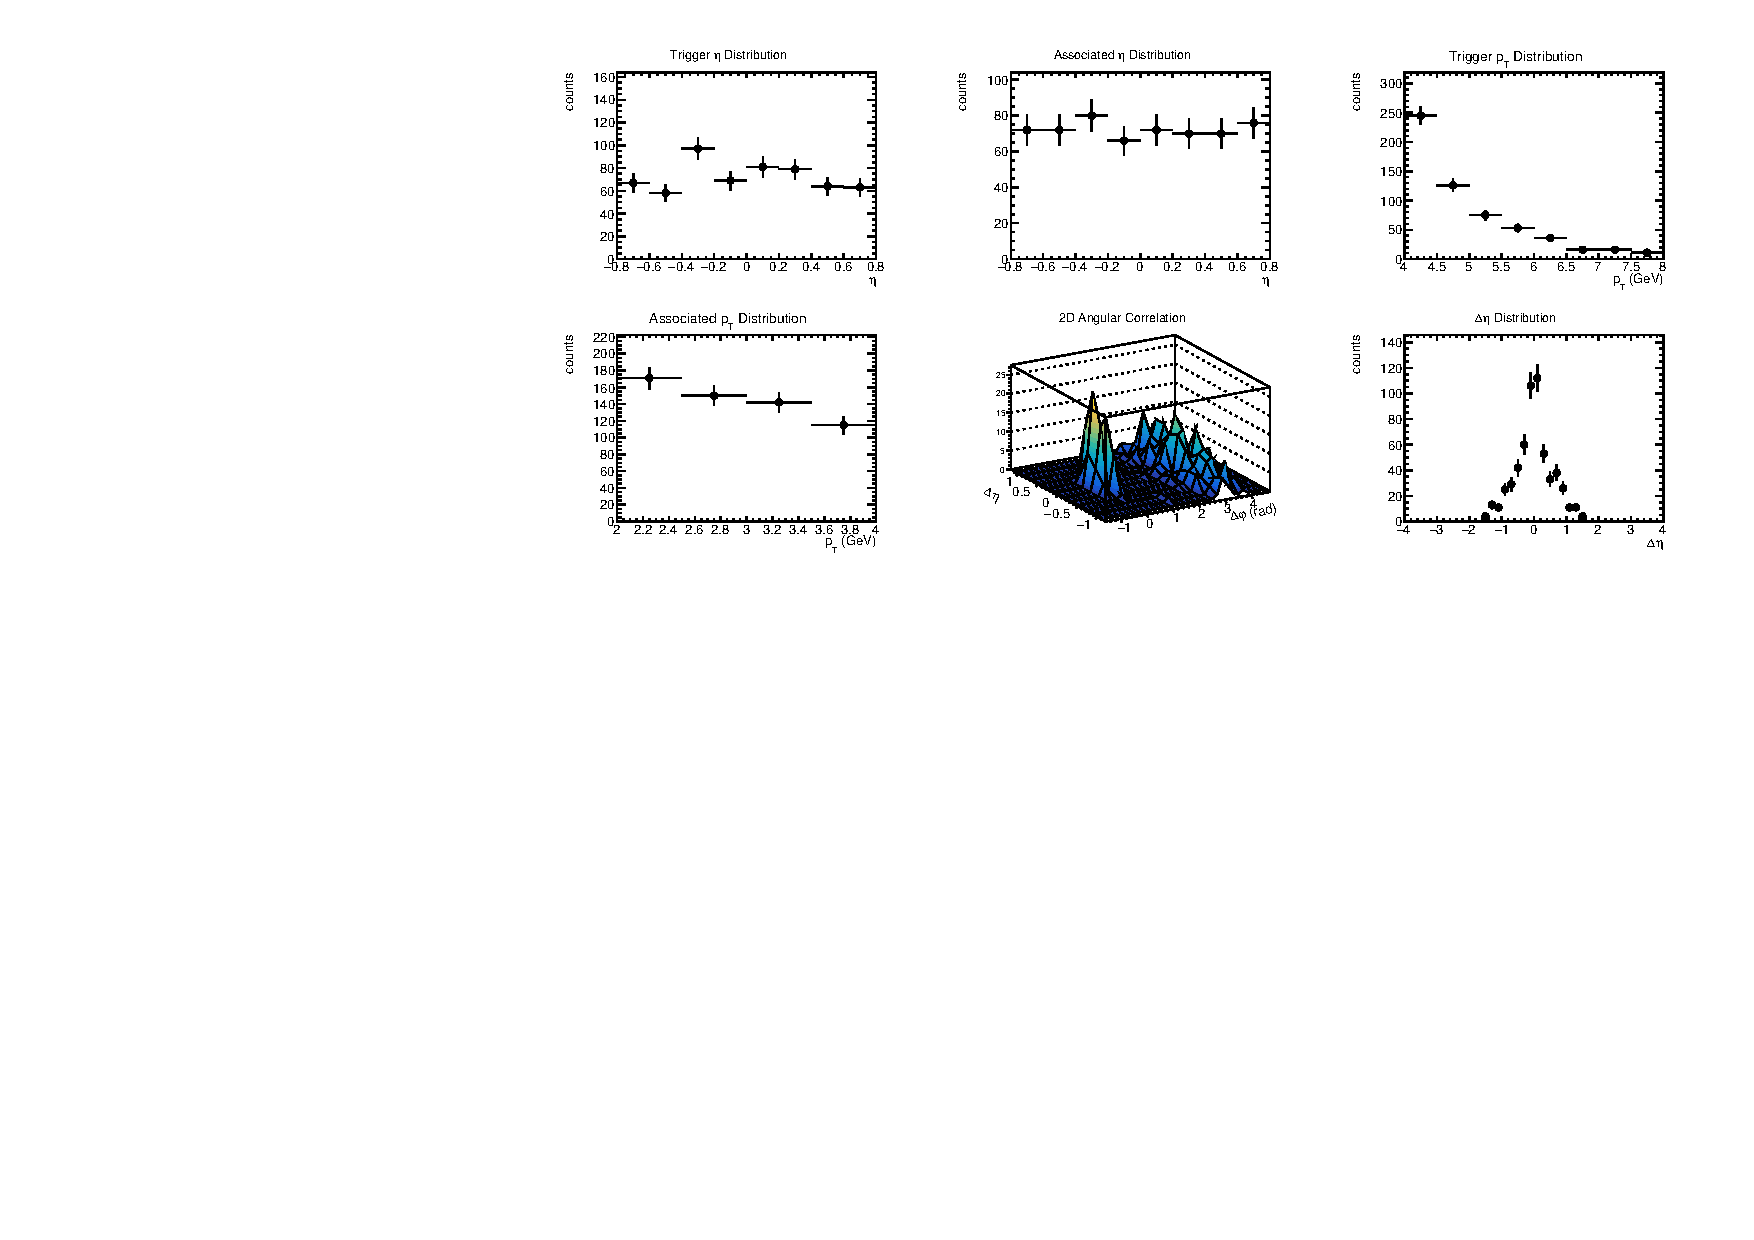
\includegraphics[scale=0.9]{results/figs/hl08_projections.pdf}
    \caption{A h---$\Lambda$ correlation for $2 < p_T^{\text{assoc}} < 4$, $4<p_T^{\text{assoc}}<8$, and $|\eta|<0.8$. Note we have much more statistics for the h---h distribution.}
    \label{fig:hl08}
\end{figure}

\FloatBarrier
\begin{figure}[h]%
    \centering
    \subfloat[\centering Trigger $p_T$ distributions.]{{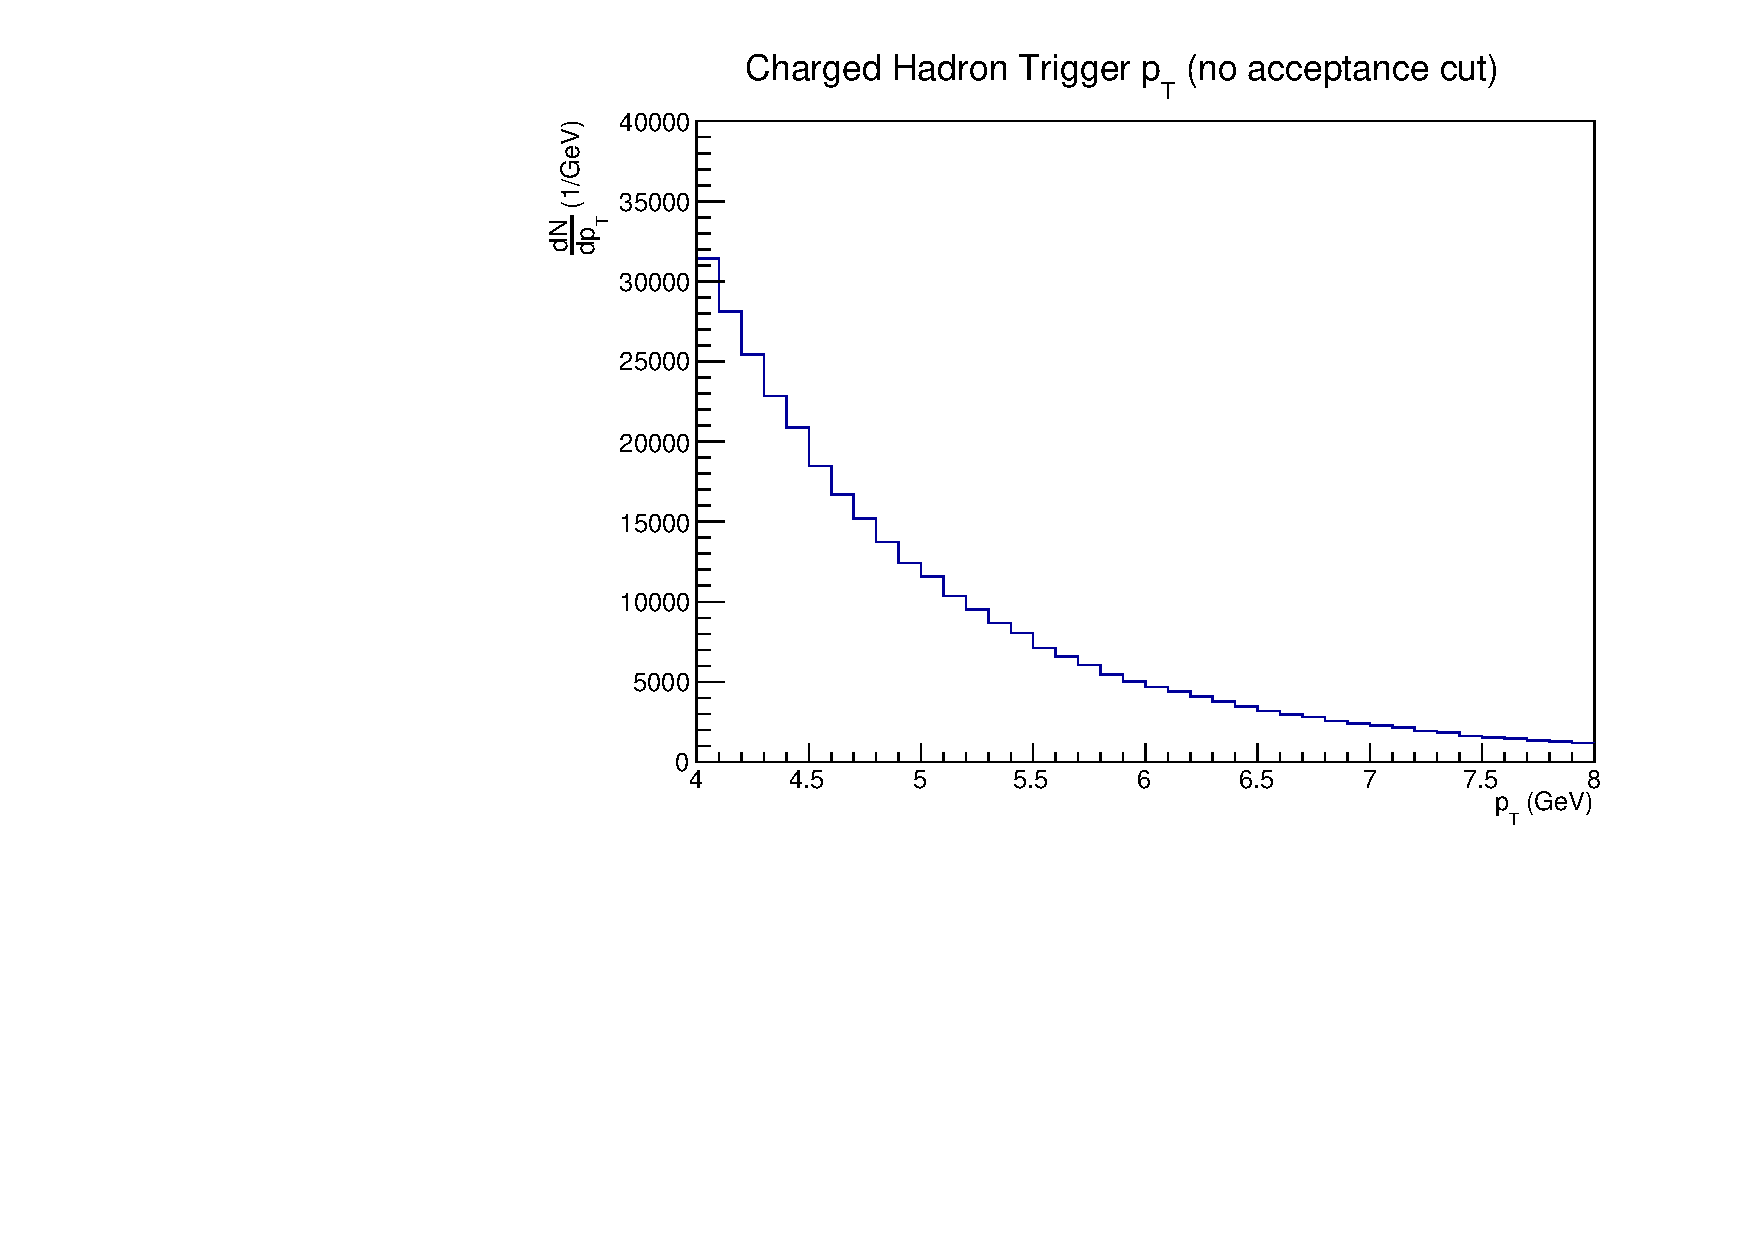
\includegraphics[scale=0.35]{results/figs/trigger_pt.pdf} }}%
    \qquad
    \subfloat[\centering Trigger $\varphi$ distribution.]{{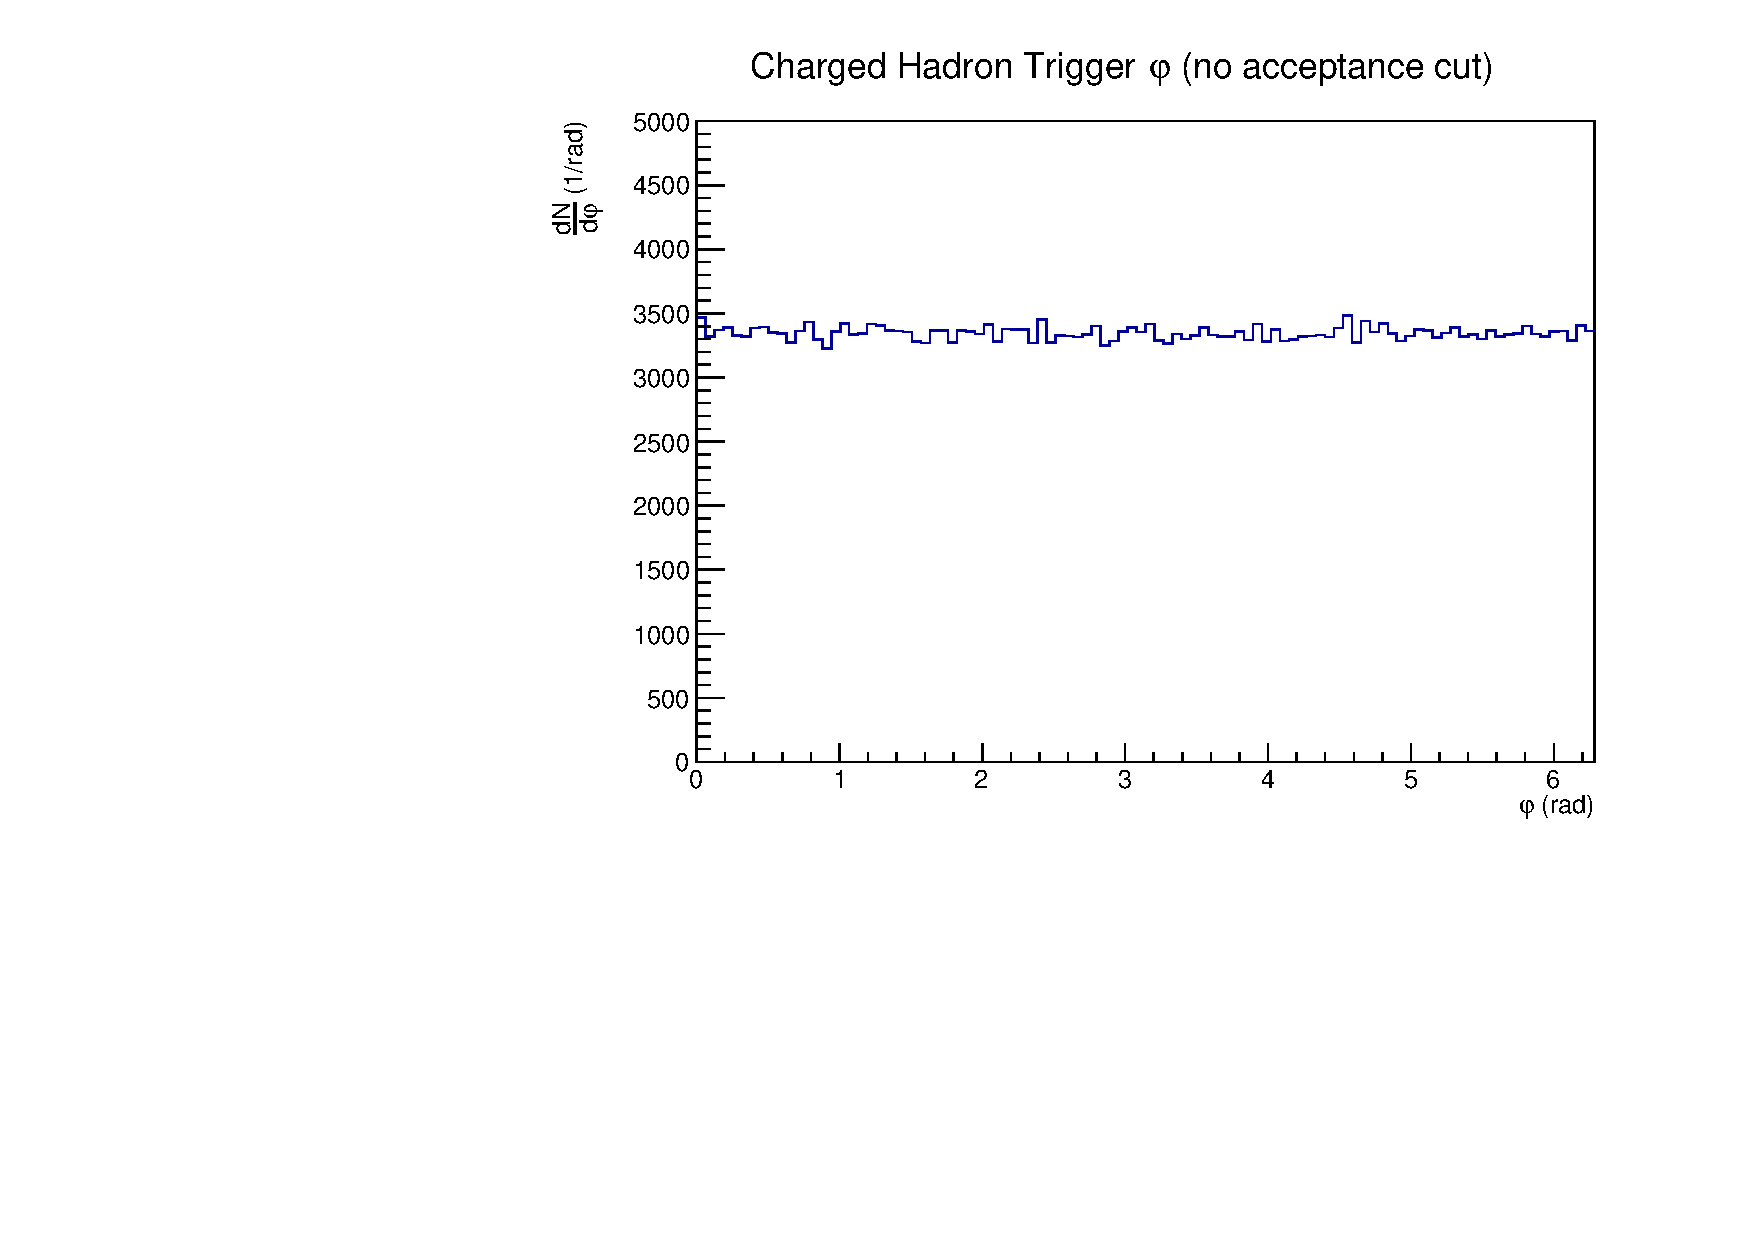
\includegraphics[scale=0.35]{results/figs/trigger_phi.pdf} }}%
    \caption{The $p_T$ and $\varphi$ distributions for all trigger hadrons. From Fig. \ref{fig:pt_dist}, we see that very few charged hadrons are within the trigger $p_T$ range.}%
    \label{fig:yield_ratios}%
\end{figure}
\FloatBarrier


\section{Yields}
The yield ratios for the near- and away-side are shown for each acceptance. These yields are a simple sum of the counts in each bin within a peak, so the uncertainty is simply the principal root of the yield. For all ratios, errors are propagated via the standard propagation of uncertainty, assuming no correlation between variables. From Fig. \ref{fig:yield_ratios}, we see the yield ratios agree across all acceptances. Thus, no systematic corrections are needed for the yield ratios. We also calculated the yield ratios for more acceptance cuts, which we include in Appendix \ref{appendix:b}. 

% \begin{figure}
% \begin{minipage}{\columnwidth}
% 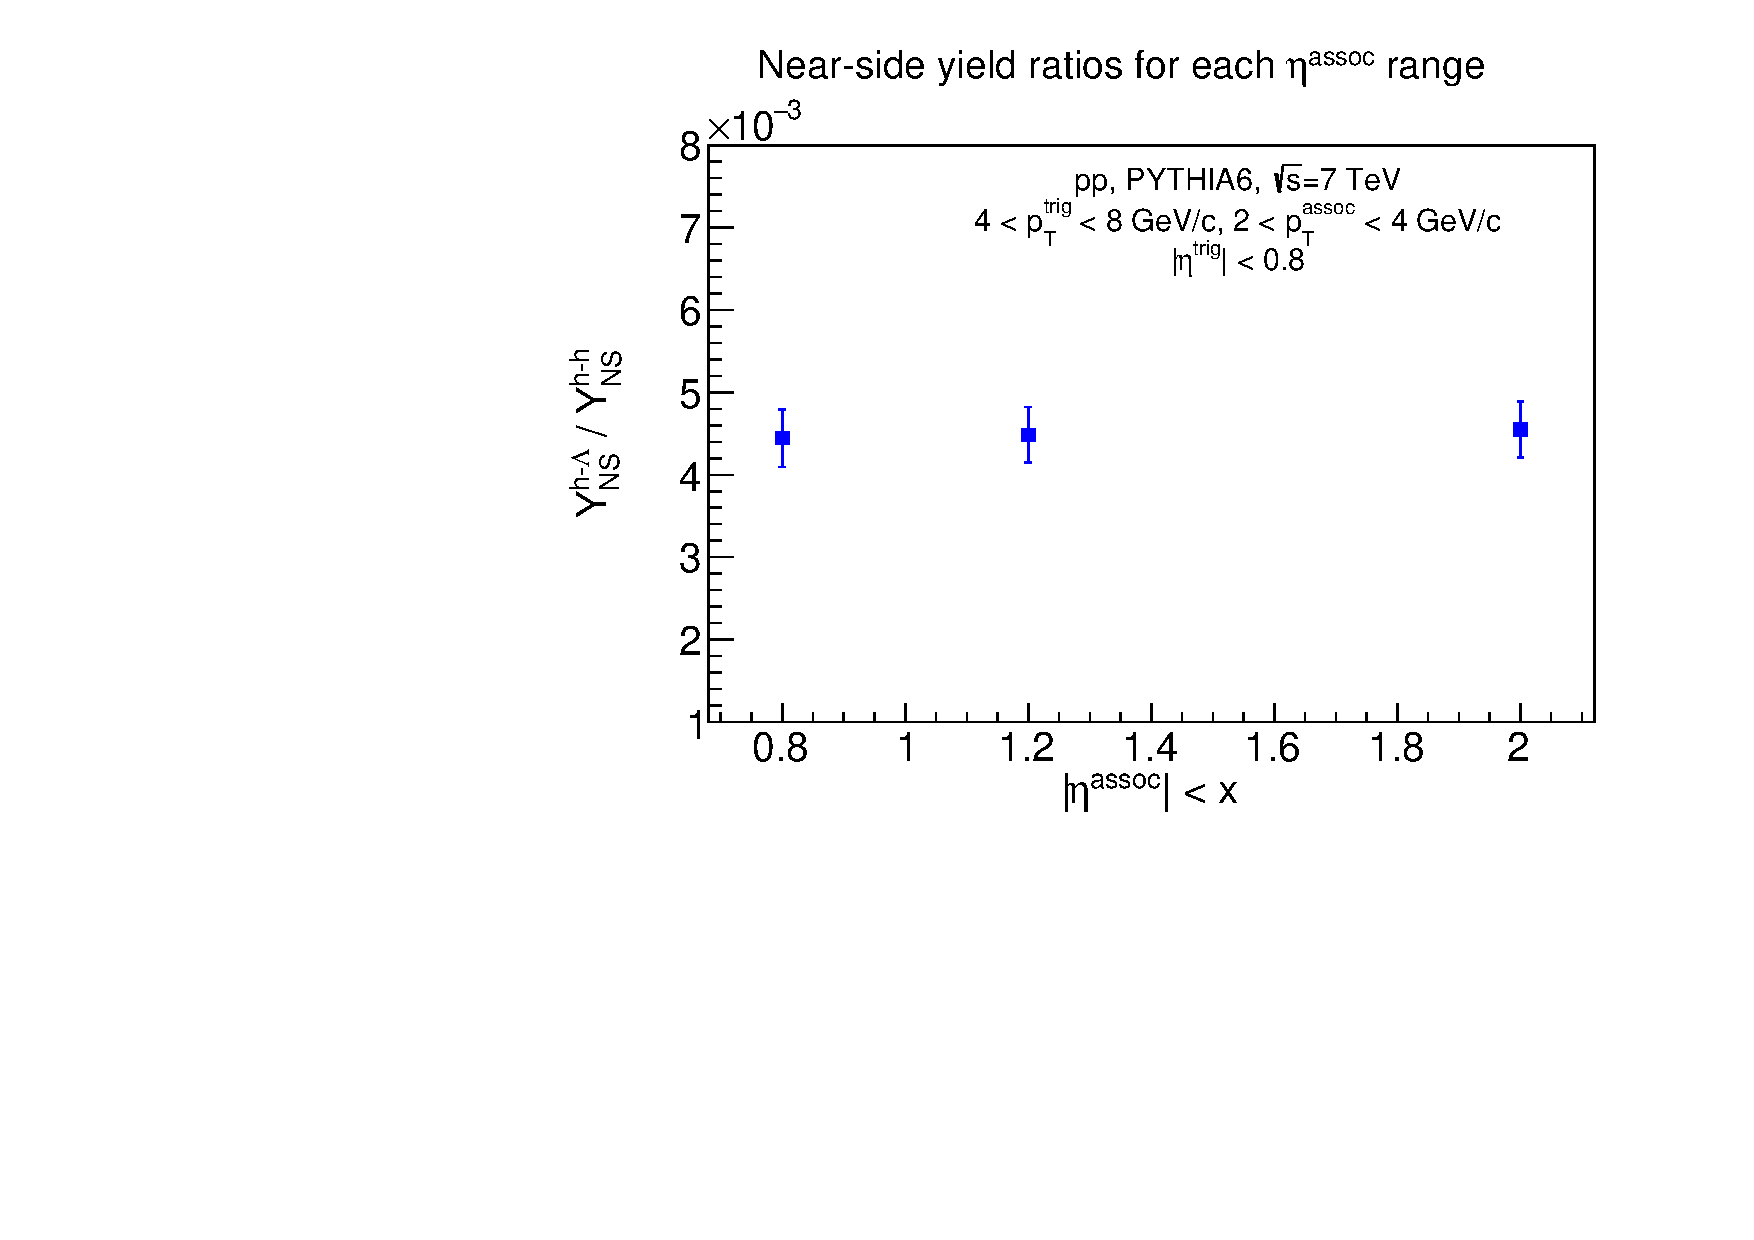
\includegraphics[width=3.0in]{results/figs/near_yield_ratios.pdf}
% \end{minipage}
% \begin{minipage}{\columnwidth}
% 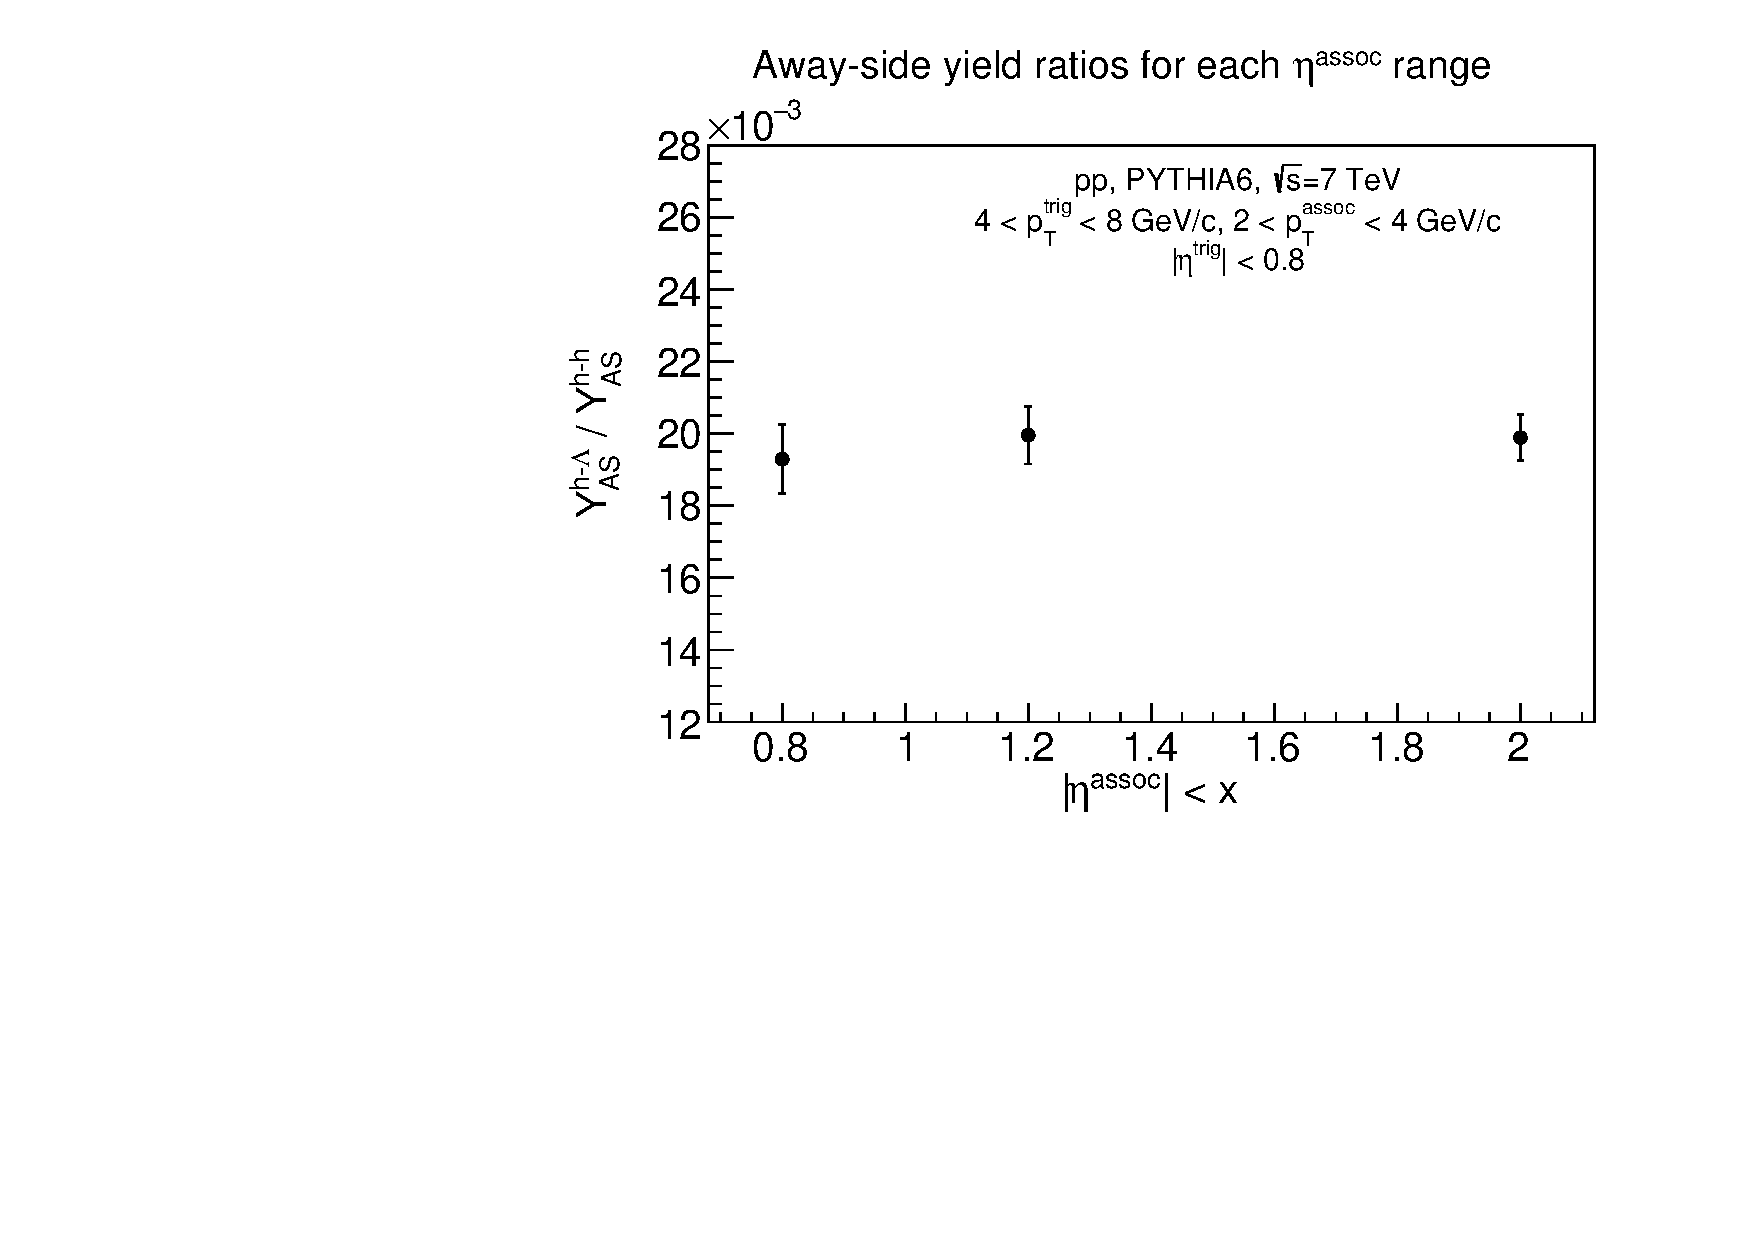
\includegraphics[width=3.0in]{results/figs/away_yield_ratios.pdf}
% \end{minipage}
% \caption{...}
% \label{two figures stacked}
% \end{figure}

\begin{figure}[h]%
   \centering
   \subfloat[\centering Near-side yield ratios.]{{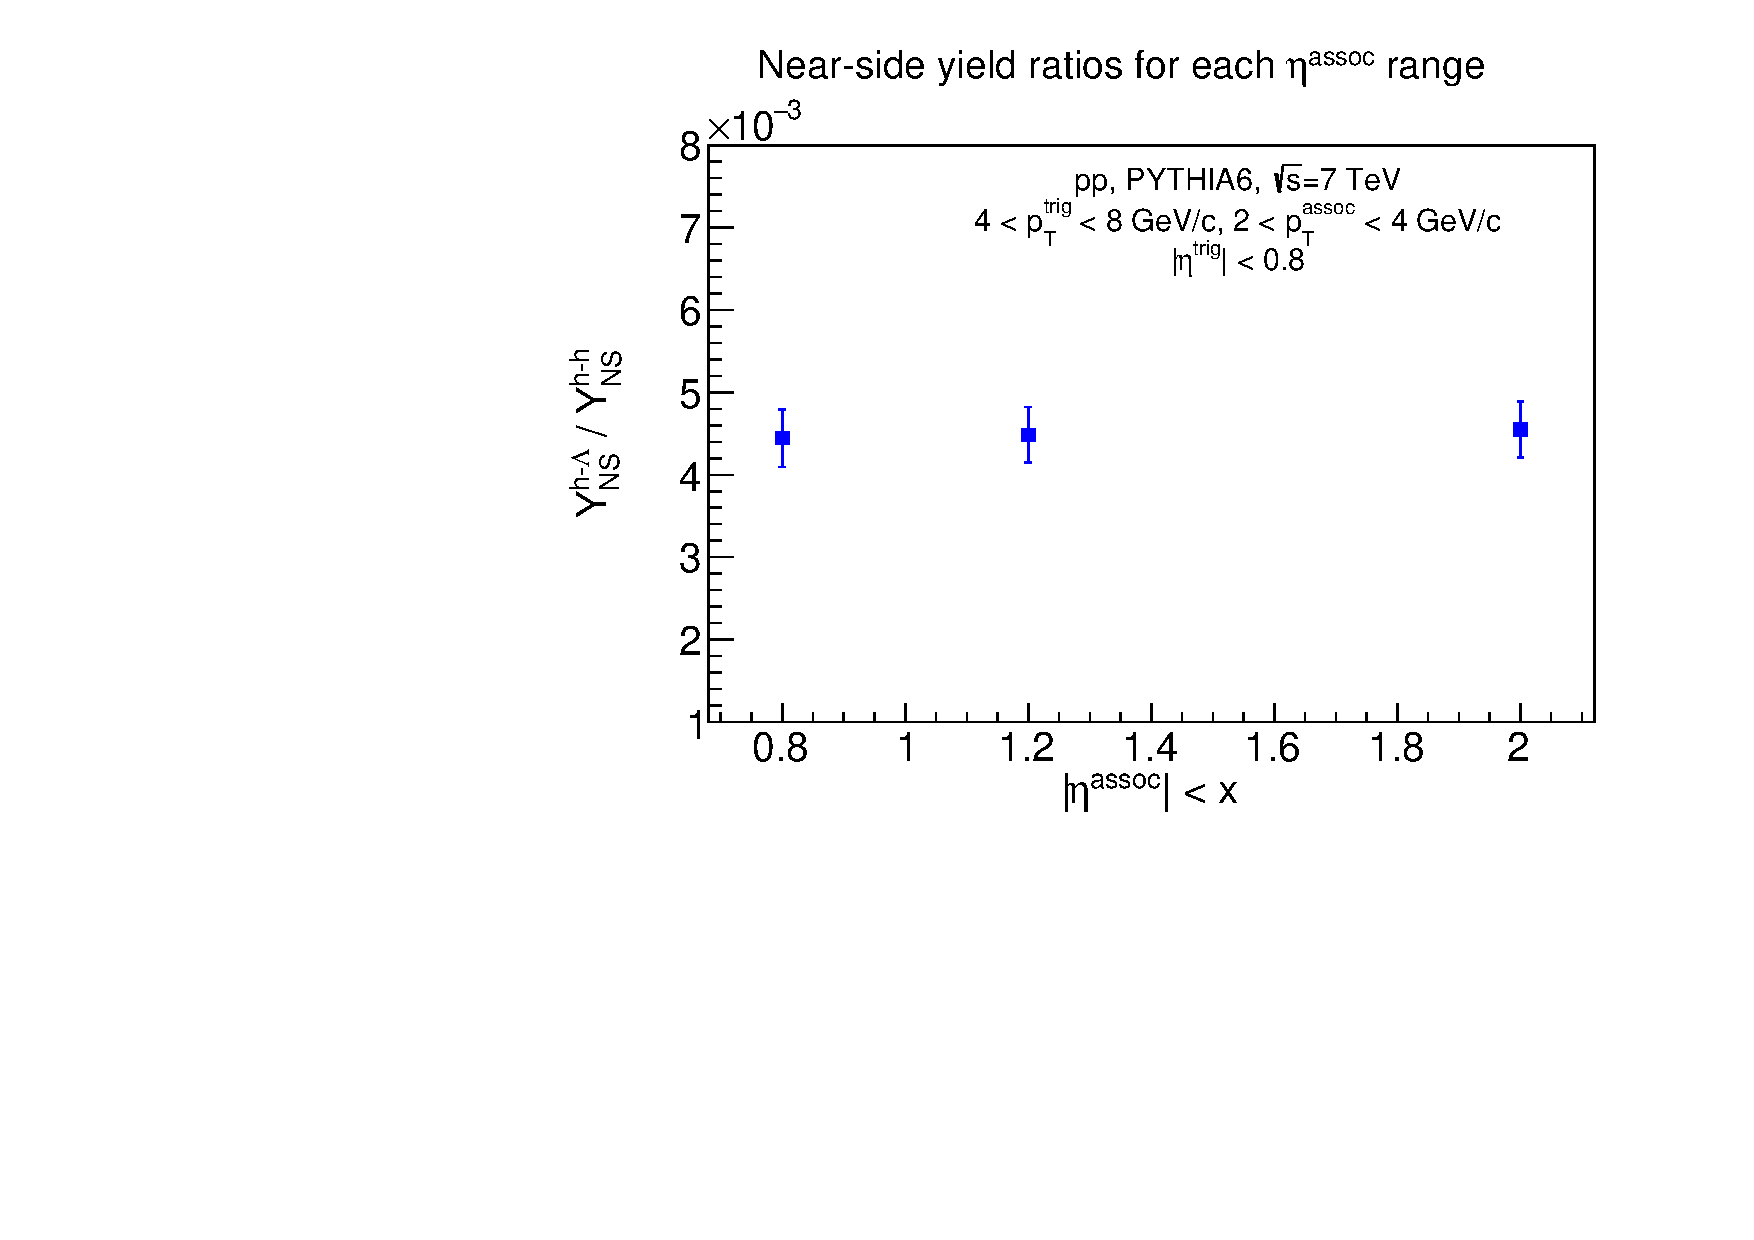
\includegraphics[scale=0.47]{results/figs/near_yield_ratios.pdf} }}%
   %\qquad
   \subfloat[\centering Away-side yield ratios.]{{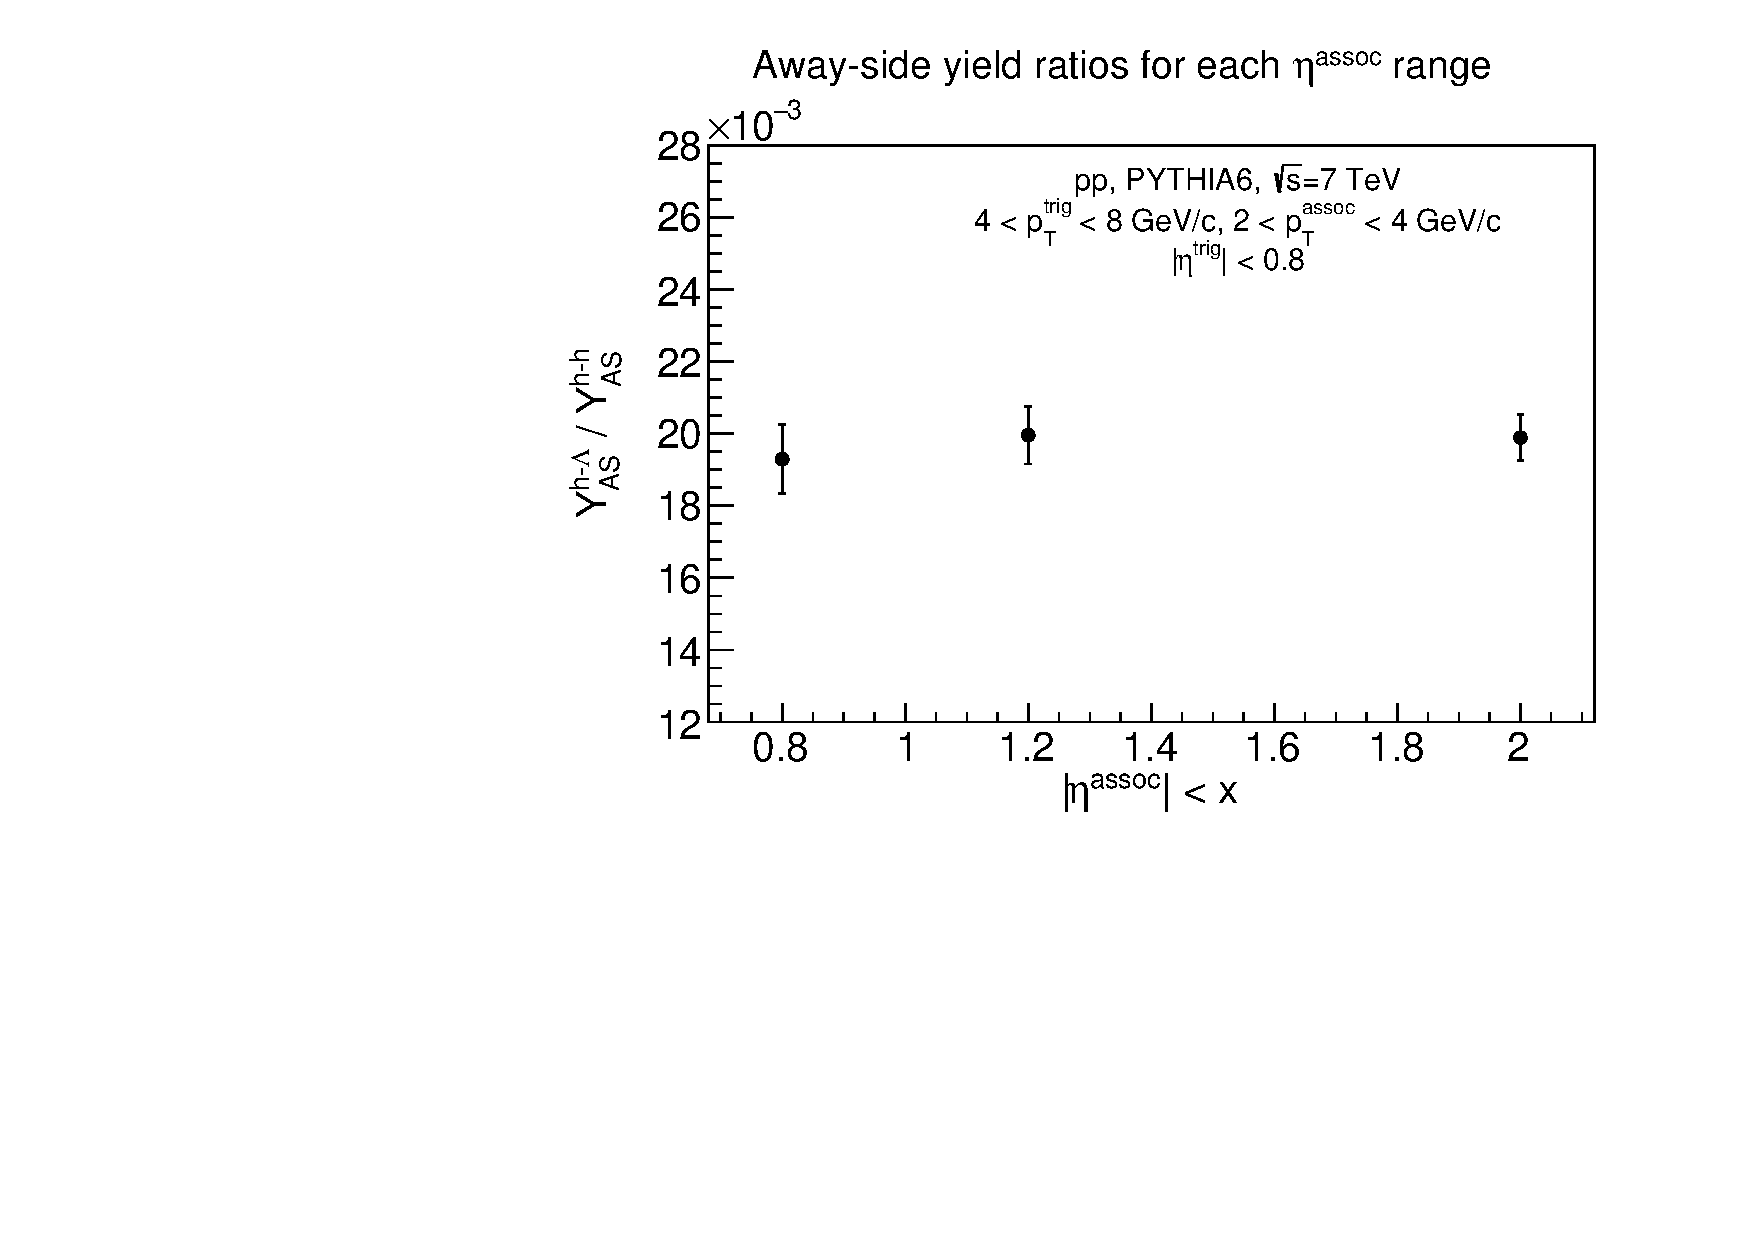
\includegraphics[scale=0.47]{results/figs/away_yield_ratios.pdf} }}%
   \caption{Yield ratios for each $\eta$ cut on the associated. Both the yield ratios on the near- and away-side agree across all cuts.}%
   \label{fig:yield_ratios}%
\end{figure}

\clearpage
\section{Widths}
The width ratios for each acceptance are presented across all acceptances in Fig. \ref{fig:width_ratios}. The width here is simply the standard deviation from the double Gaussian fit. We see the width ratios agree for all acceptances, indicating no further systematic corrections are required. For each distribution, we also calculate the ratio of the away-side to near-side width (Fig. \ref{fig:as_over_ns}). The near-side is chosen as the normalization since the trigger serves as the jet-axis proxy. In addition, the away-side is quenched in heavy-ion collisions, so normalizing by the near-side lets us compare. We find a slight downward trend for both the h---$\Lambda$ and h---h correlations as the acceptance is opened, although more statistics are needed to make a robust physics interpretation. The downward trend suggests the away-side broadens more slowly than the near-side. Since a tight cut on $\eta$ modifies the $p_T$ spectrum by introducing a bias towards midrapidity, this trend could result from a $p_T$ dependence. 


\begin{figure}[h]%
    \centering
    \subfloat[\centering Near-side width ratios.]{{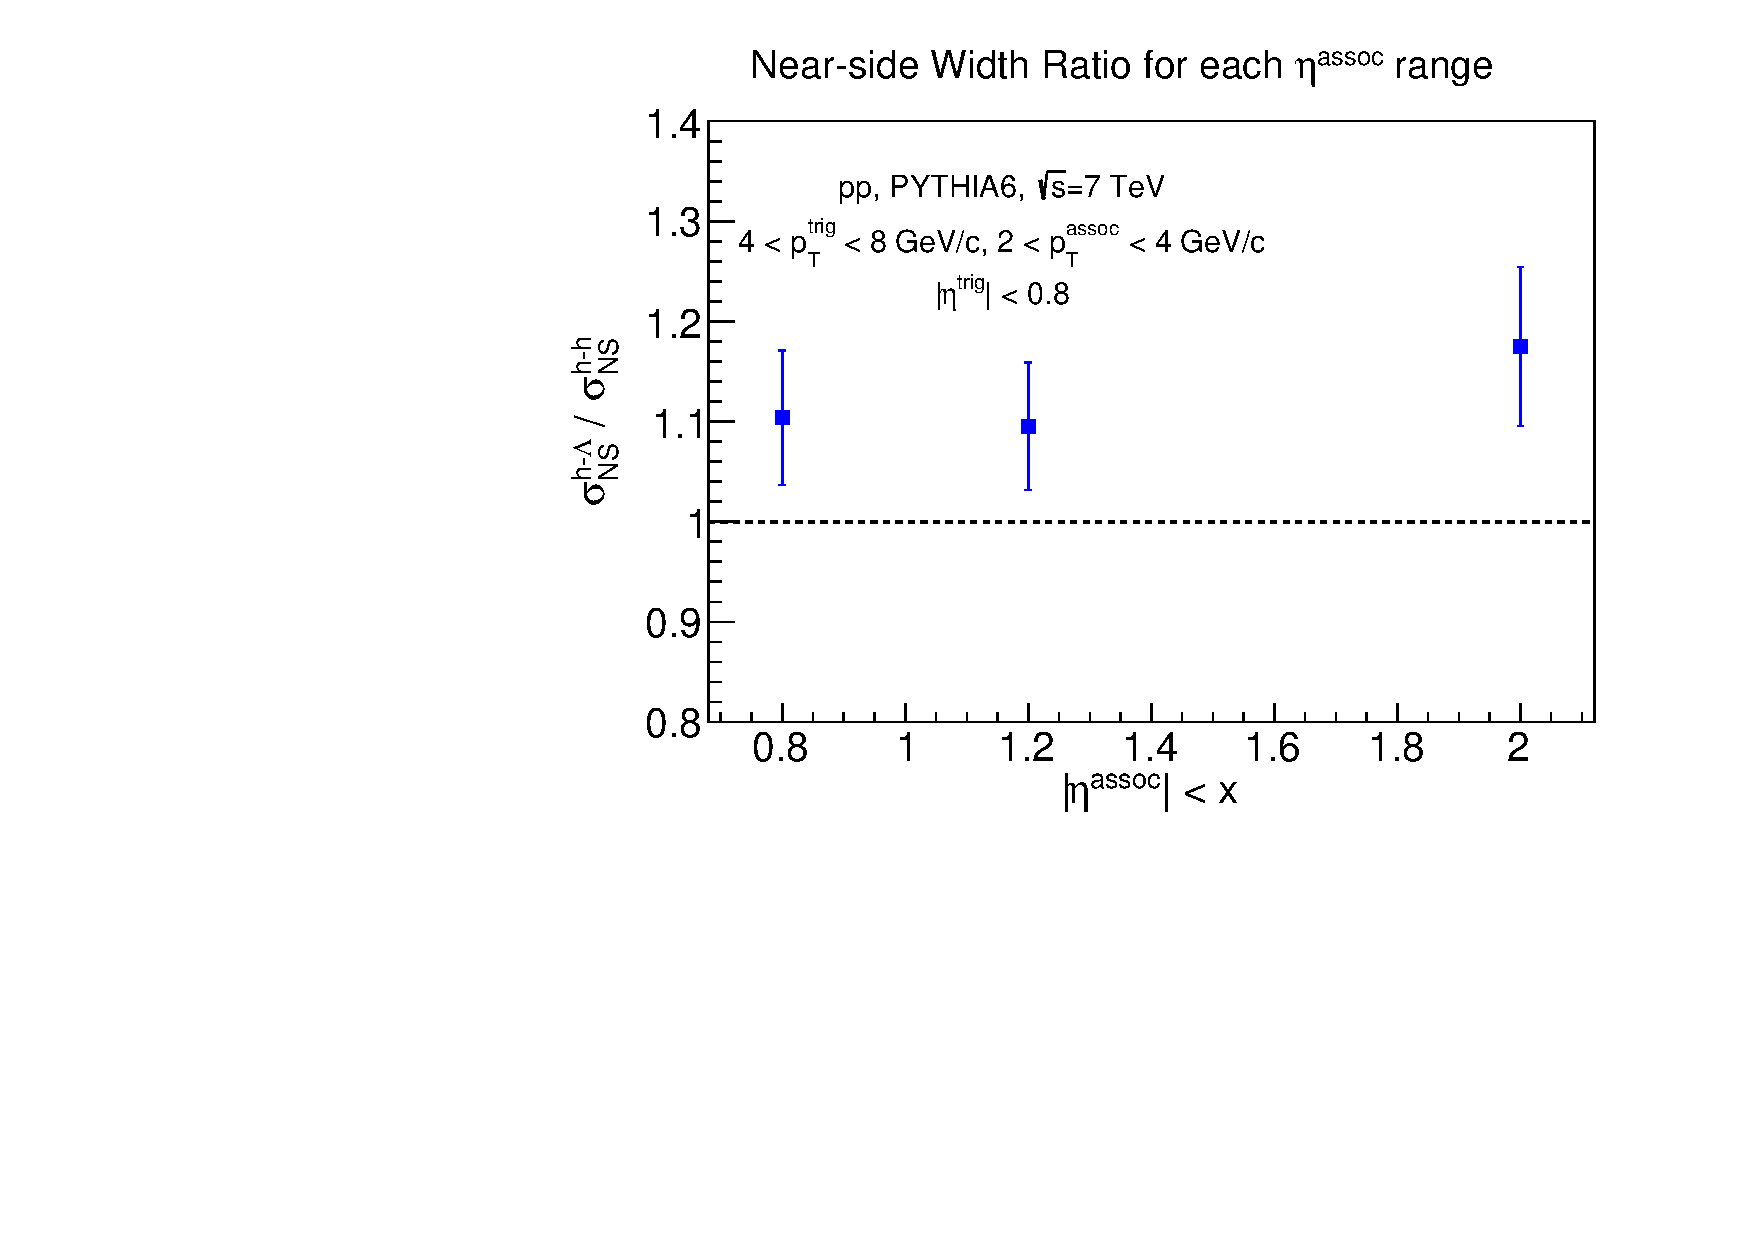
\includegraphics[scale=0.45]{results/figs/near_side_width_ratios.pdf} }}%
    %\qquad
    \subfloat[\centering Away-side width ratios.]{{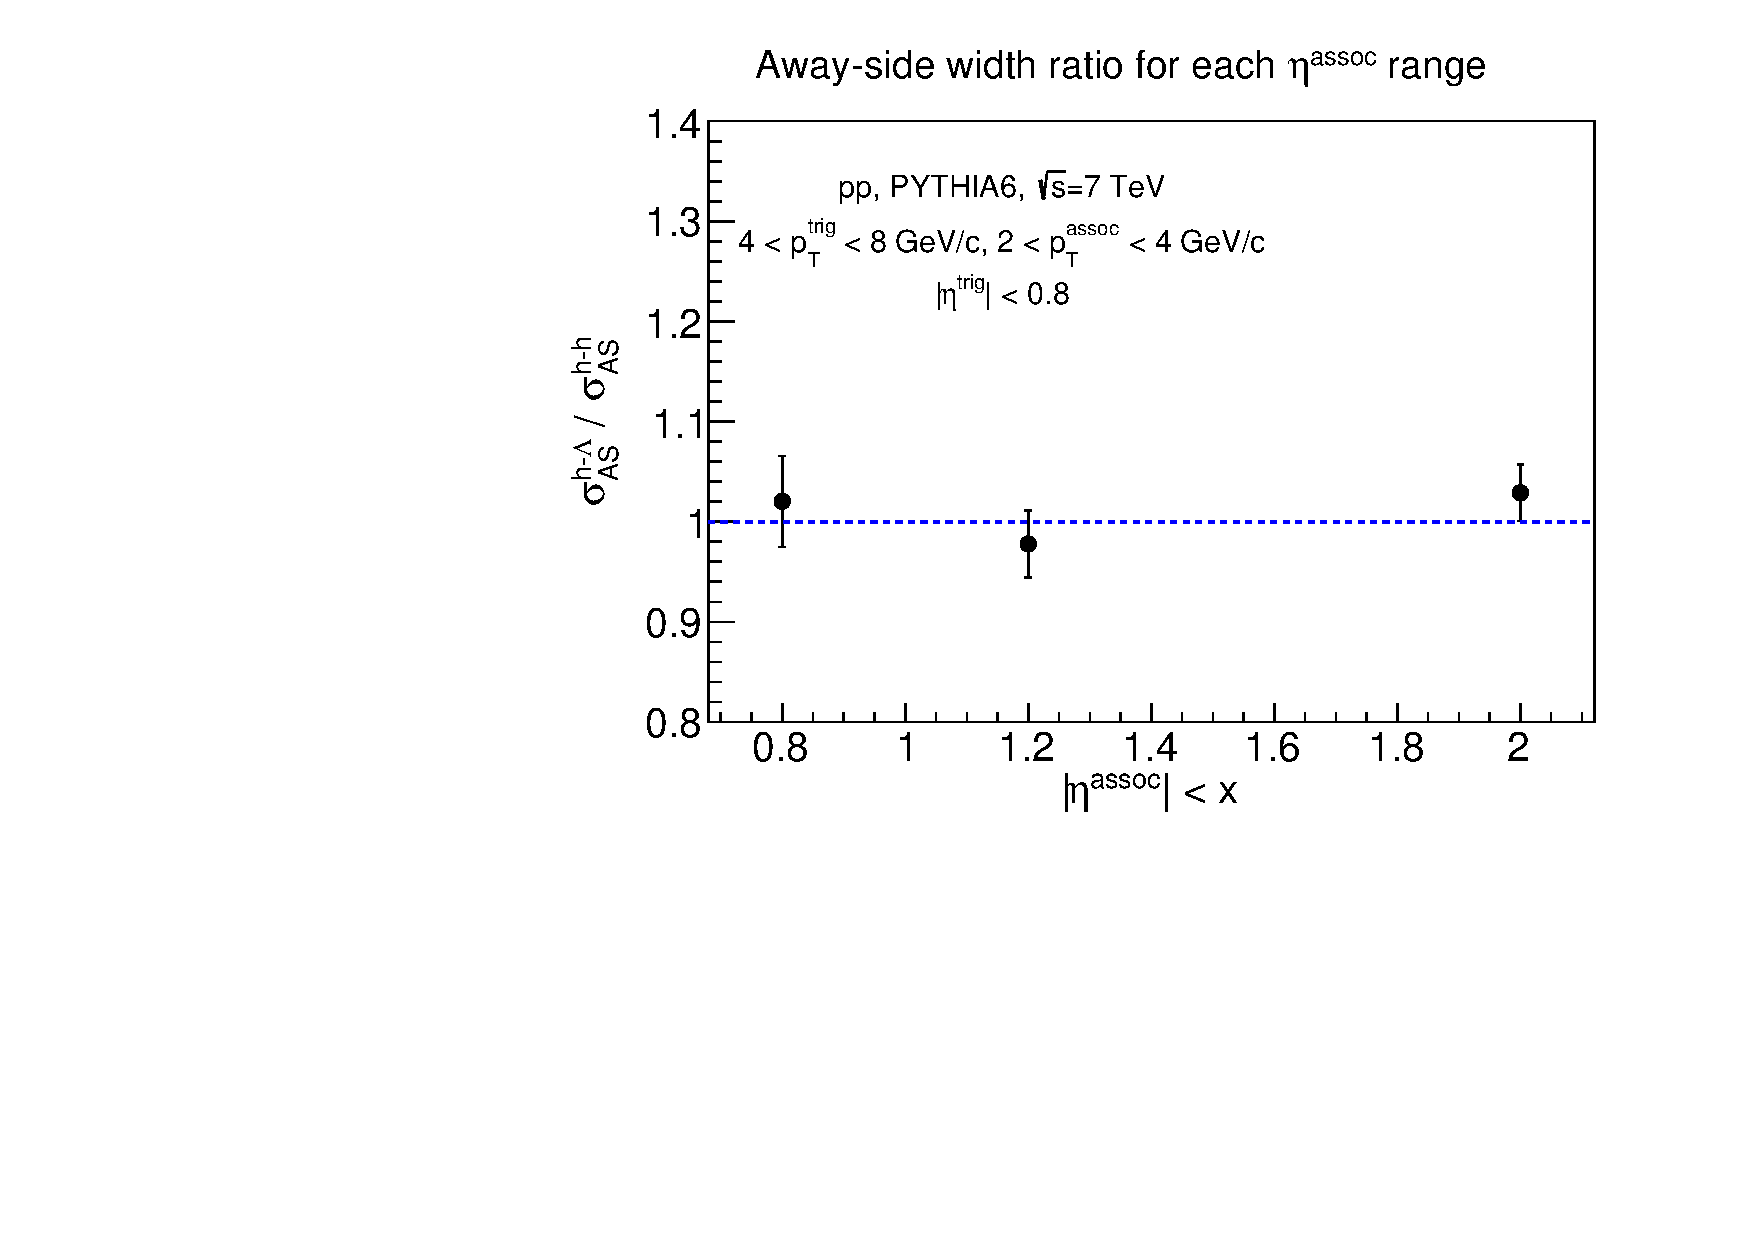
\includegraphics[scale=0.45]{results/figs/away_side_width_ratios.pdf} }}%
    \caption{Width ratios for each $\eta$ cut on the associated. Both the width ratios on the near- and away-side agree across all cuts.}%
    \label{fig:width_ratios}%
\end{figure}

\FloatBarrier
\begin{figure}[h]
    \centering
    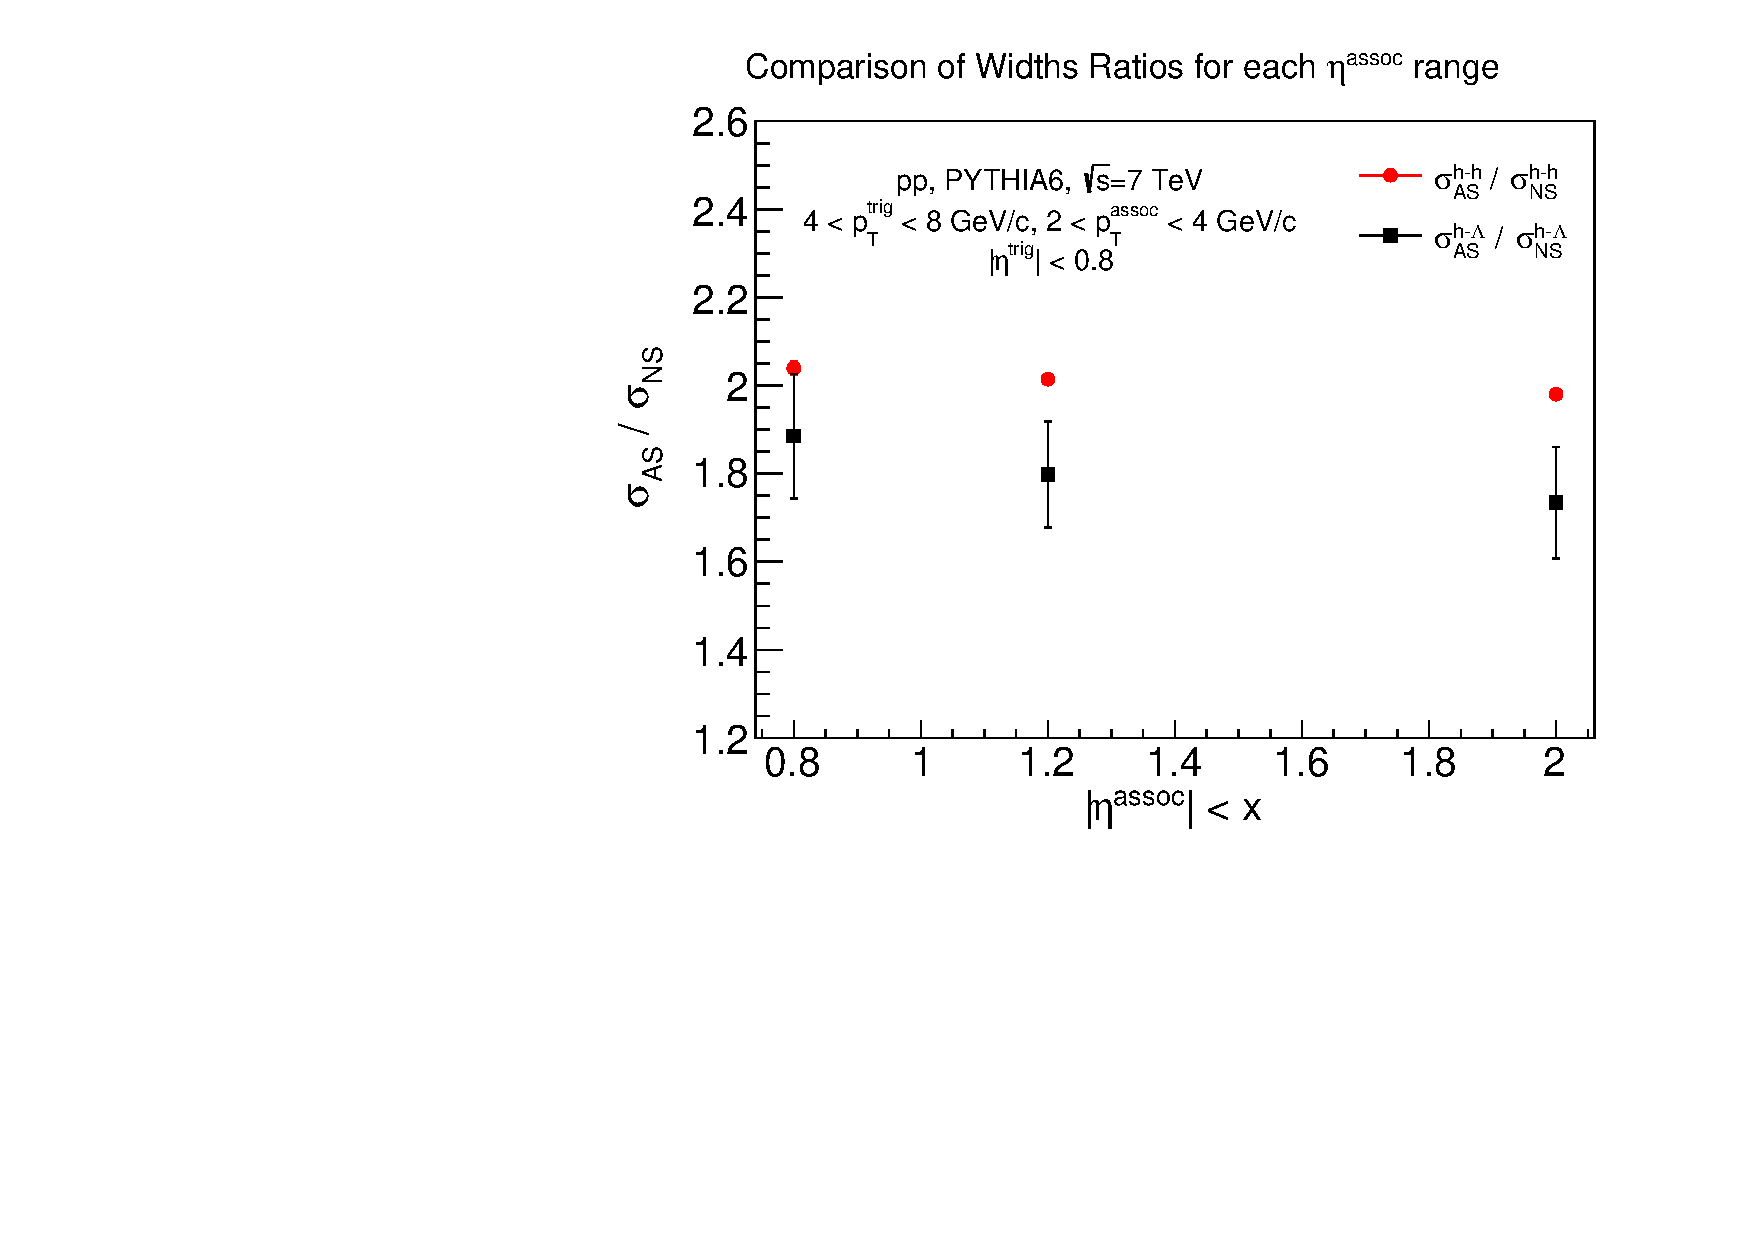
\includegraphics[scale=0.5]{results/figs/away-over-near.pdf}
    \caption{Near-side widths over away-side widths for each $\eta$ cut and distribution.}
    \label{fig:as_over_ns}
\end{figure}
\FloatBarrier

\section{Evaluation of Fit Stability}
All experiments and analyses involve choices; even if they are good choices, they can impact results in subtle ways. Systematic errors attempt to quantify these uncertainties that do not arise from statistical fluctuations. Since the choice of fit function is somewhat arbitrary, we must ensure the extracted widths truly reflect the spread of each peak. The Gaussian function seems like a good choice since it is quite common and seems simpler than the generalized Gaussian and Von Mises, but there is no obvious reason to choose the Gaussian. As a systematic check, we also calculate widths and width ratios using the generalized Gaussian and Von Mises. If these widths and ratios are in general agreement, we can be confident in the values we assign to the widths---this is a systematic check. All fits are included in Appendix \ref{appendix:a}, and an example of the various fit functions is shown in Fig. \ref{fig:fit_examples}. 


\begin{figure}[h]
    \centering
    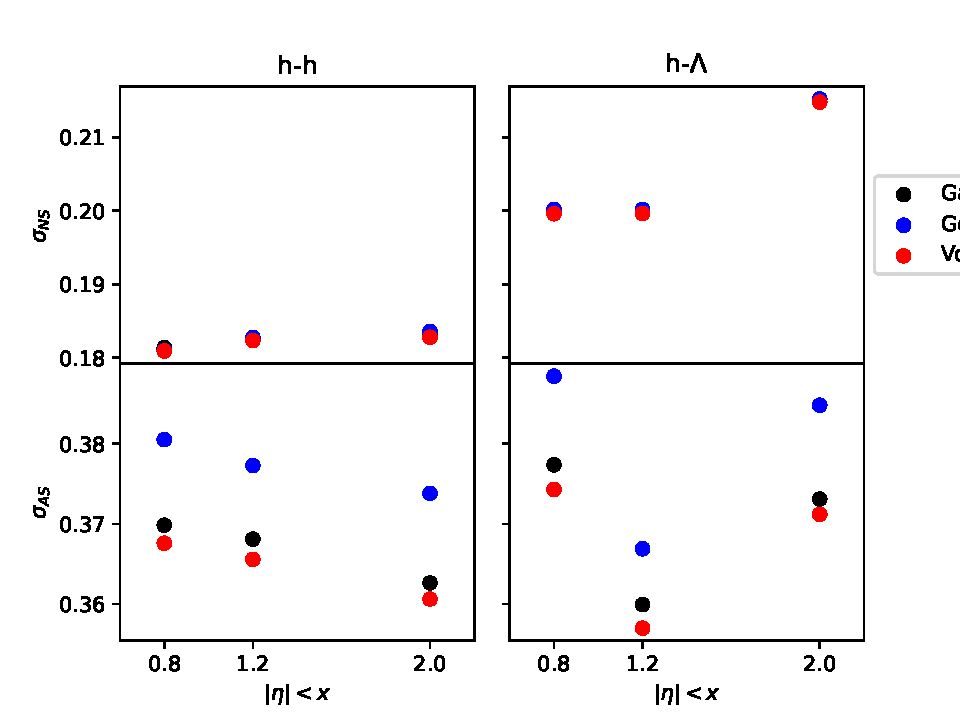
\includegraphics[scale=0.7]{results/figs/widths-across-fits.pdf}
    \caption{Near- and away-side widths for each fit function and distribution. We see the widths are in general agreement. Note the vertical axes do not start at zero.}
    \label{fig:fit_widths}
\end{figure}

We show the fitted widths from each fit function across acceptances in Fig. \ref{fig:fit_widths} and the corresponding width ratios in Fig. \ref{fig:fit_ratios}. The results are quite close between all fits, indicating that our fits are stable. In Fig. \ref{fig:fit_widths}, the value of $\sigma$ agrees for all fits on the near-side, and h---$\Lambda$ away-side. For the away-side of the h---h distribution, the generalized Gaussian predicts consistently higher widths than the Von Mises and Gaussian distributions. A close inspection of the fits reveals the h---h away-side is slightly triangular, which the generalized Gaussian can capture with its flexibility in shape. The errors on the widths calculated from the generalized Gaussian are consistently larger than those from the Gaussian and Von Mises fits. This is likely an overestimate of the error and requires closer inspection. This could result from a correlation between $\alpha$ and $\beta$, meaning we would need to account for more elements of the covariance matrix when propagating errors. We suspect this is an overestimate because the calculated width ratios are extremely close. Any disagreement in the measure of the absolute widths cancels in the ratios. Thus, we use the Gaussian distribution for our final results because it is the "simplest" distribution. In reality, this choice is arbitrary but does not affect the interpretation that our acceptance cut does not artificially modify our correlations.  


\begin{figure}[h]
    \centering
    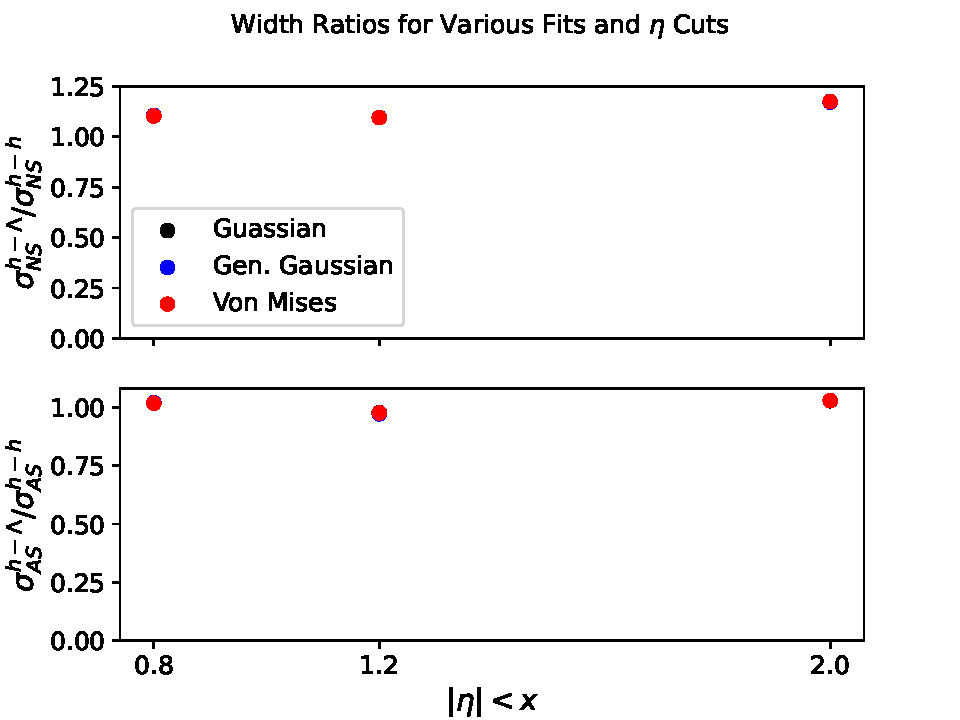
\includegraphics[scale=0.7]{results/figs/ratios-across-fits.pdf}
    \caption{Near- and away-side width ratios for each fit function and distribution. The horizontal axis represents each of the three $\eta$ cuts. We see the fits mostly agree and any disagreement cancels in the width ratios.}
    \label{fig:fit_ratios}
\end{figure}

In many fits shown in Appendix \ref{appendix:a}, the $\chi^2/\text{NDF}$ values are lower for the h---$\Lambda$ distributions. At face value, this indicates a better fit; however, we must consider that there are many more high $p_T$ hadrons than $\Lambda$ hyperons. Consequently, the relative uncertainty in each bin of our h---h distributions is much lower than for the h---$\Lambda$ correlation. Due to larger uncertainties, a fit can describe the h---$\Lambda$ distribution much more easily, and the $\chi^2$ value is driven down. On the other hand, a fit must describe the h---h distributions exceptionally well for the $\chi^2$ to not blow up due to minuscule uncertainties. We expect the fits of the h---$\Lambda$ correlations would worsen with more statistics. From a physics standpoint, fragmentation need not produce Gaussian correlations, and our h---h distributions are certainly not entirely Gaussian. We only use fit functions that are Gaussian-like, so we should expect similar extracted widths. In other words, the fact that our width ratios are similar across fit functions does not necessarily indicate goodness-of-fit. This is a potential weakness that could be addressed with a different choice of fit function. However, since the fits are stable and generally capture the width of near- and away-side, we can still interpret the widths of our correlations. We find that the width ratios are not affected by acceptance, given the choice of fit. 


\section{Future Work}
We would like to further investigate strangeness production by comparing simulations of p-Pb to data. While p-p events offer a good baseline to isolate acceptance-dependent effects, we can still learn much more about strangeness enhancement in p-Pb. In particular, we are interested in the event generator Parton-Hadron-String Dynamics (PHSD), which aims to capture the microscopic aspects of events \cite{Cassing:2009vt}. In PHSD, we aim to study how strangeness production differs for various types of strange hadrons.   
 

\ifSubfilesClassLoaded{%
    \printbibliography
}

\end{document}